\chapter{An'alisis y Dise'no de la aplicaci'on m'ovil}
\label{capituloseis}
En el presente c'apitulo se describe el desarrollo de la aplicaci'on m'ovil para cumplir con el objetivo general de \textit{proveer servicio a trav'es de una aplicaci'on m'ovil}. 
El desarrollo de la aplicaci'on m'ovil es la secuencia de pasos para ofrecer como resultado una aplicaci'on m'ovil.

Para el desarrollo de la aplicaci'on m'ovil se aplic'o el modelo iterativo incremental porque ha facilitado la comprensi'on y el analisis para el avanze de la aplicaci'on m'ovil en una serie de pasos hacia una soluci'on en diversas versiones hasta producir un aplicaci'ion adecuado\cite{Somerville2011}.

%\section{Estructura del Proyecto}
%\label{EstructuraIonic}
Para la estructura del proyecto utiliza el framework ionic con la  estructura de modelo, vista y controlador. Esta estructura se genera autom'aticamente al momento de crear el proyecto en carpetas y archivos para organizar el c'odigo. La estructura del framework se desarrolla en el anexo \ref{estructuraIonic}.


%\section{Implementaci'on del Proyecto}
%La implementaci'on se ha realizado seg'un los modulos \ref{ModuloMovil}, el dise'no de interfaz \ref{DisenoMovil} se han realizado en el c'apitulo \ref{capituloseis} y las herramientas de la aplicaci'on movil que se ha desarrollado en el c'apitulo \ref{capitulodos} los cuales  se dividen en las siguientes iteraciones.
Para el desarrollo de la aplicaci'on m'ovil se tiene informaci'on de la recolecci'on de datos del capitulo \ref{capitulotres} y la etapa de crear un nuevo servicio en el capitulo \ref{capitulocinco}.

\section{Primera iteraci'on}
En la primera iteraci'on se realizo la lista de requerimientos, el dise'no de interfaz  y la implementaci'on con datos estaticos.

\subsection{La primera etapa de analisis}
Como se ha mencionado anteriormente la informaci'on para la recoleccion de datos se obtuvo de los capitulos \ref{capitulotres} y \ref{capitulocinco}. El resultado es la siguiente lista de requerimientos.
%La especificaci'on de los requerimientos se tiene a partir del requerimiento del servicio en el c'apitulo \ref{capitulocinco} en la secci'on de requerimientos \ref{requerimientoServicio} y con la recolecci'on de datos del c'apitulo \ref{capitulotres} para cumplir el objetivos general de \textit{proveer los servicios de la aplicaci'ion SAGAA a trav'es de una aplicaci'on m'ovil}.
\textbf{Lista de requerimientos}
\begin{itemize}
\item Realizar Dise'no adaptativo.
\item Realizar la sesi'on.
\item Listar la gesti'on.
\item Listar carreras.
\item Mostrar los datos de la planilla de notas
\item Modificar la planilla de notas.
\item Almacenar la planilla de notas en el celular. 
\item Modificar planilla de notas sin internet.
\end{itemize}

Despu'es de concluir con la lista de requerimientos realizamos el dise'no para mostrar los datos de la planilla de notas.

\subsection{La primera etapa de dise'no interfaz}
\label{Doc:Interfaz}
El dise'no de interfaz representa el como se muestran los datos de la planilla de notas es por este motivo que tiene algunos datos repetidos como se muestra en la figura \ref{fig:IU}.
\begin{figure}[H]
\centering
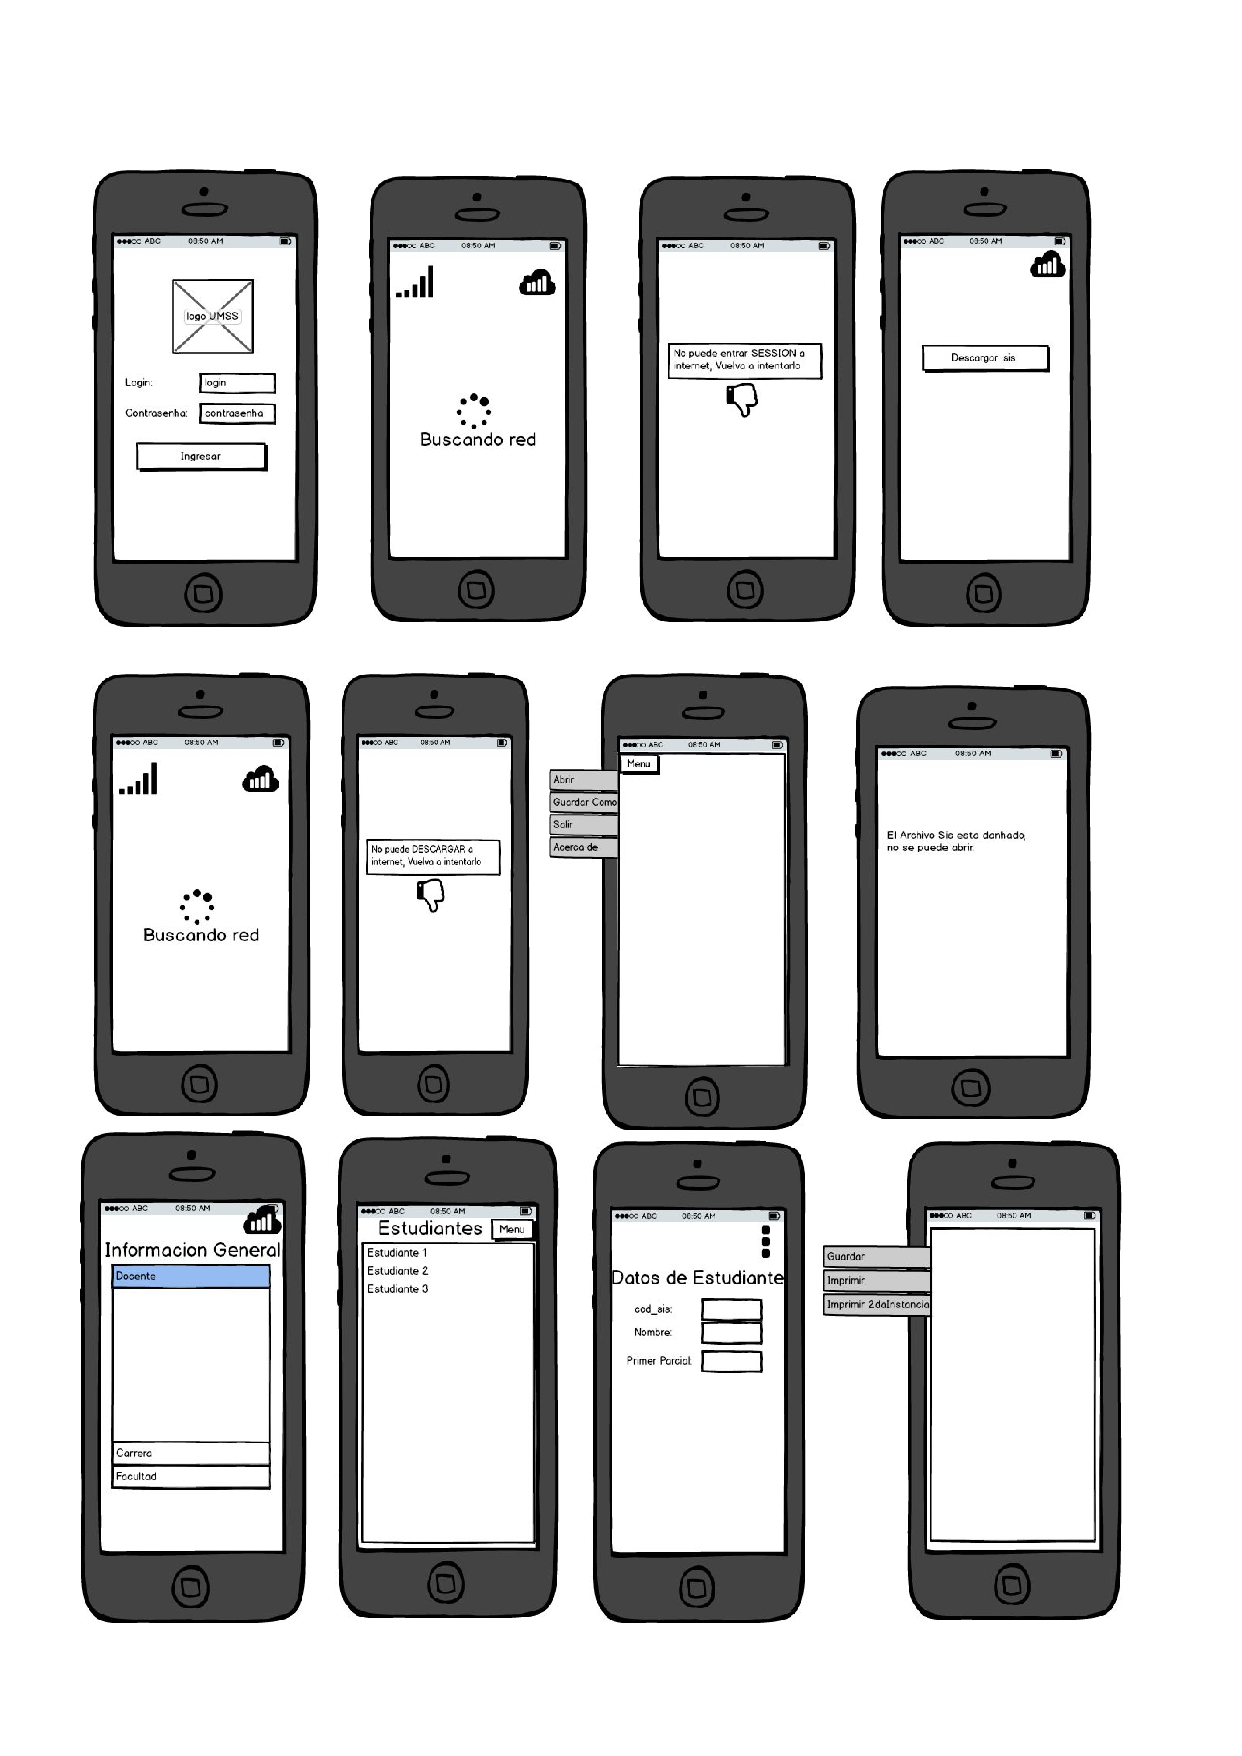
\includegraphics[width=0.6\textwidth]{mockupimprimir.pdf}
\captionsetup{justification=centering,margin=2cm}
\caption{Interfaz de Usuario primera etapa, Fuente: Elaboraci'on Propia}
\label{fig:IU}
\end{figure}

La interpretaci'on de la informaci'on de la planilla de notas es el primer paso para el desarrollo de la aplicaci'on m'ovil.

\subsection{La primera etapa de la implementaci'on}
Para la implementaci'on primeramente interpreta la informaci'on de la planilla de notas y gracias a la herramienta extra json y otros. Lo importante en la implementaci'on es la siguiente linea de c'odigo.
\begin{itemize}
\item Ordenar los datos del servicio web, se realizo en el archivo www/js/fileService.js en donde ordena los datos de la planilla de notas.

\begin{verbatim}
divFile : function(data , template){
if(template == 'informacion'){
   	return (((((data.pcd).head)[0]).info))[0];
	.........
},
crearBDInf : function(array){
	return  newBD = {
    	'fechaC ' : array[0],
        'fechaE'  : array[1],
        'codDoc' : array[2],
        'nomApeDoc' : array [3],
        ..........
    };
},
\end{verbatim}
\end{itemize}
  
\section{Segunda iteraci'on}
En la segunda etapa de iteraci'on se especifica el desarrolla de los m'odulos y el dise'no de la comunicaci'on con el servicio.

%\subsection{Dise'no de la comunicaci'on entre cliente y servicio}
%El dise'no de la comunicaci'on es una representaci'on abstracta de las solicitudes o peticiones que realiza la aplicaci'on m'ovil(cliente) y las respuestas del servicio web ofrece, como se muestra en la figura \ref{fig:DCS}.

%\begin{figure}[H]
%\centering
%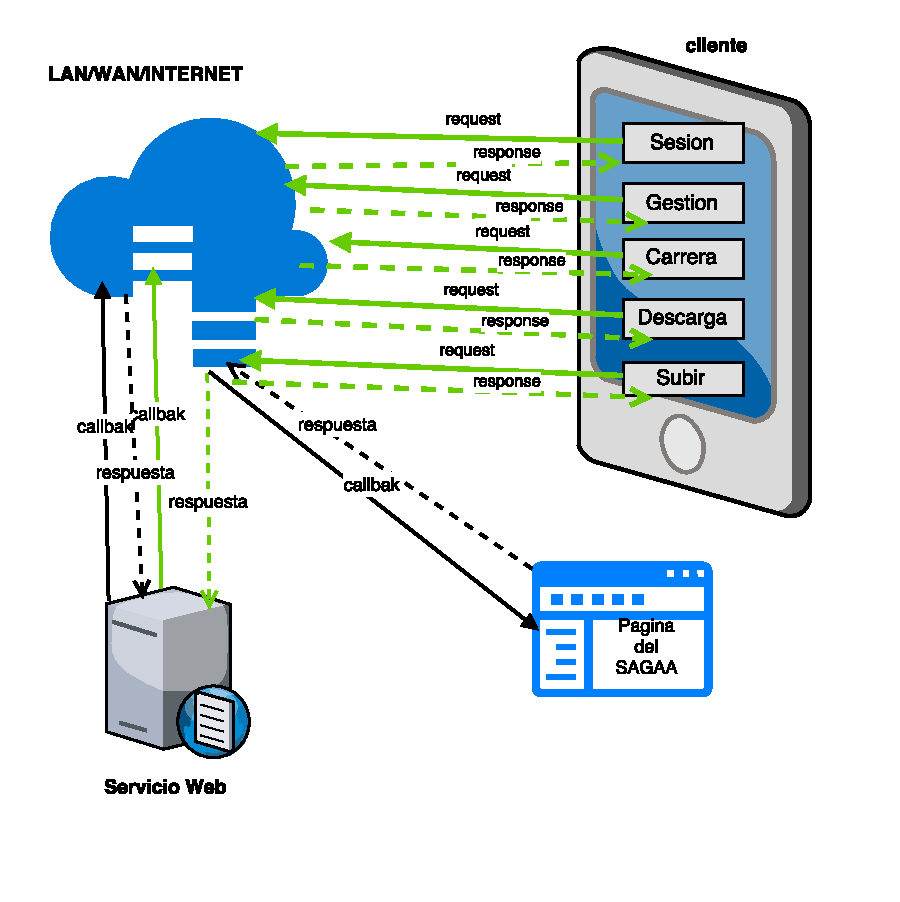
\includegraphics[width=0.4\textwidth]{comunicacionCS.pdf}
%\captionsetup{justification=centering,margin=2cm}
%\caption{Dise'no de comunicaci'on entre el cliente y servicio web Fuente: Elaboraci'on Propia}
%\label{fig:DCS}
%\end{figure}

%La implementaci'on es el proceso de realizar el dise'no como una aplicaci'on movil, que se explica a continuaci'on.

\subsection{La segunda etapa del analisis}
\label{ModuloMovil}
A partir de la lista de requerimientos se realiza el an'alisis de la segunda etapa, en esta etapa a continuaci'on se realiza la lista de m'odulos y subm'odulos las cuales son: 

\subsection{Lista de m'odulos del proyecto}
\begin{enumerate}
\item Mostrar la planilla de notas.
\item Modificar la planilla de notas.
\item Obtener datos del servicio web.
\item Guardar la planilla de notas en el servicio web.
\end{enumerate}
     
\subsection{ Lista de submodulo del proyecto}
\begin{enumerate}
\item Mostrar la planilla de notas.
\begin{itemize}
\item Crear la sesi'on para mostrar la planilla de notas.
\item Seleccionar la planilla de notas seg'un la gesti'on.
\item Seleccionar la planilla de notas seg'un la carrera.
\end{itemize}

\item Modificar la planilla de notas.
\begin{itemize}
\item Mostrar la planilla de notas ordenado por grupo.
\item Modificar la planilla de notas por grupo.
\end{itemize}

\item Obtener datos del servicio web.
\begin{itemize}
\item Verificar la sincronizaci'on con el servicio web.
\item Si no tiene sincronizaci'on con el servicio web generar un repositorio de la planilla de notas local.
\end{itemize}

\item Guardar la planilla de notas en el servicio web.
\begin{itemize}
\item Enviar la planilla de notas al servicio web.
\item Verificar la sincronizaci'on con el servicio web para guardar la planilla de notas.
\end{itemize}
\end{enumerate}

Una vez concluido con la lista de m'odulos se determina el dise'no de interfaz para la aplicaci'on m'ovil.

\subsection{ La segunda etapa del Dise'no de interfaz }
\label{DisenoMovil}
El dise'no de interfaz es la etapa de proceso donde las m'odulos y subm'odulos se interlazan con la implementaci'on.
%Para cumplir con el objetivo especifico \ref{sec:oe}  y se utilizan las herramienta de wireframe, las cuales son:

El segundo dise'no se ha modificado con las observaciones del primer intento y se toma en cuenta el servicio. El dise'no se presenta en la en la siguiente figura \ref{fig:IU2}.

\begin{figure}[H]
\centering
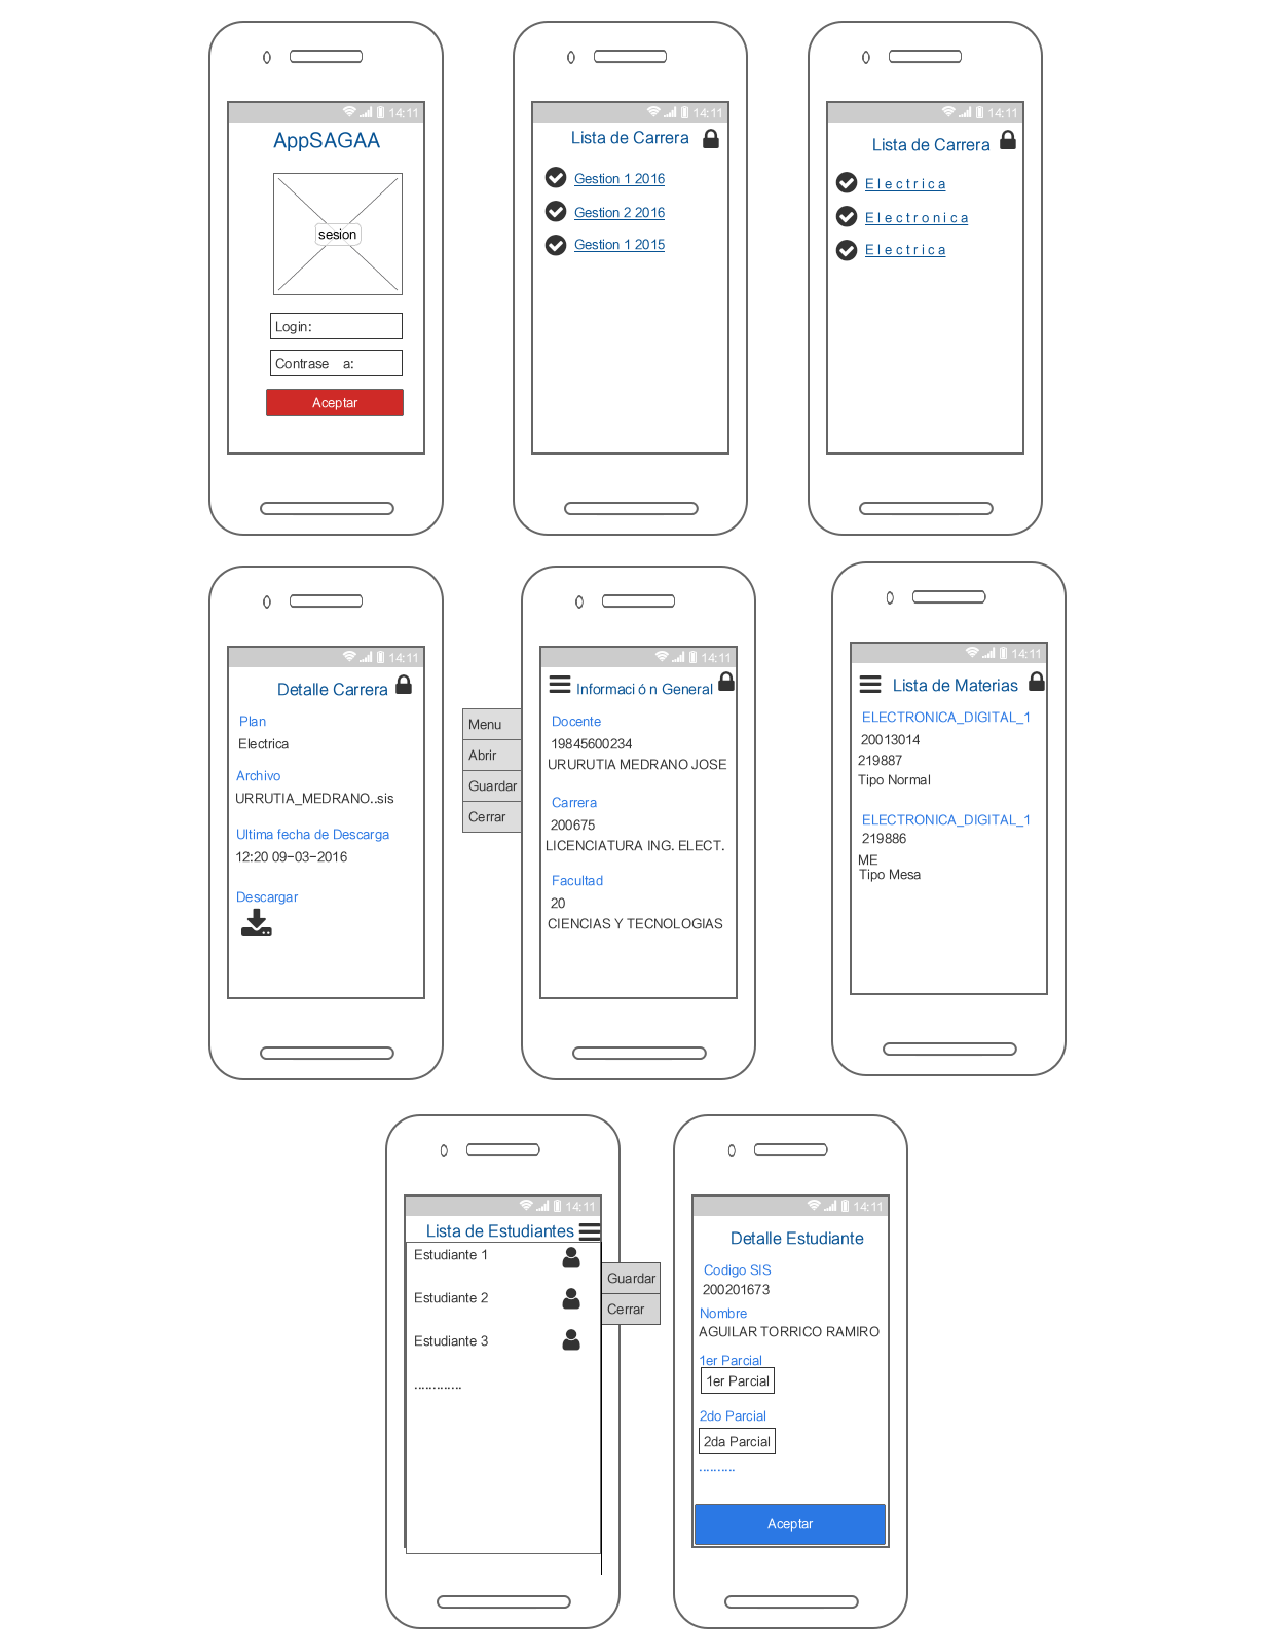
\includegraphics[width=0.5\textwidth]{Interfaz.pdf}
\captionsetup{justification=centering, margin=2cm}
\caption{Interfaz de Usuario representado en mockups, Fuente: Elaboraci'on Propia}
\label{fig:IU2}
\end{figure}
\end{enumerate}
  
Una vez concluido con el dise'no de interfaz, conocido como el esquema de pantallas, se desarrolla la implementaci'on.
%, se realiza el dise'no de la comunicaci'on entre cliente y el servicio web.

\subsection{La segunda etapa de la Implementaci'on}
En esta etapa de implementaci'on se desarrolla la comunicaci'on con el servicio, la sesi'on a traves del servicio, solicitar informaci'on del servicio y otros. En los siguientes indicen se explican algunos de la implementaci'on.

\begin{itemize}
\item Solicitud de la planilla de notas al servicio web se realizo en el archivo www/js/fileFactory.js

\begin{verbatim}
sisFactory.posDataDetalle = function(carrera){
.......
 $http.post(urlBase+'/detalle', descargarD, {skipAuthorization : false}, conf).
 success(function(data) {
 .......
 }; 
\end{verbatim}

\item La configuraci'on para enviar el jwt en la cabecera de la petici'on se crea un nuevo interceptor el c'ual se guarda localmente se implemento en el archivo www/app.js

\begin{verbatim}
...
.config(function($stateProvider, $urlRouterProvider, $authProvider, 
$httpProvider, jwtInterceptorProvider, jwtOptionsProvider) { 
.....
 jwtOptionsProvider.config({
 	//IP de la maquina actual 
	 whiteListedDomains: ['localhost', '172.20.10.3'] 
	 tokenGetter: function(options, jwtHelper){
	 var token = localStorage.getItem('id_token');
}});
	//metodo para enviar un json web token
$httpProvider.interceptors.push('jwtInterceptor');
......
\end{verbatim}
\item La configuraci'on para conectar la aplicaci'on m'ovil al servicio web se ha desarrollado en el archivo www/js/fileFactory.js: 
\begin{verbatim}
//IP de la maquina donde se encuentra el server.js
var urlBase = 'http://172.20.10.3:8080';
var conf = {
	headers : {
	'Access-Control-Allow-Origin' : '*',
    'Access-Control-Allow-Methods' : 'POST, GET, OPTIONS, PUT',
    'Content-Type': 'application/jsonr',
    'Accept': 'application/json'
    } 
};
\end{verbatim}
\end{itemize}

\section{Tercera iteraci'on}
En la tercera iteraci'on se desarrolla el modificar la planilla de notas sin conexi'on a internet de la aplicaci'on movil, almacenar informaci'on en la aplicaci'on m'ovil y otros. En este iteraci'on se ha desarrollado el dise'no responsive para la aplicaci'on, el cual se explican en el c'apitulo \ref{capituloocho}.
\subsection{La tercera etapa de dise'no}
En la tercera etapa de dise'no se representa la comunicaci'on entre la aplicaci'on movil y la base de datos como se muestra en la siguiente figura \ref{fig:DO}. Como es una base de datos no sql es por este motivo que se guardan los datos como documentos por lo tanto no se tiene un dise'no de base de datos.

\begin{figure}[H]
\centering
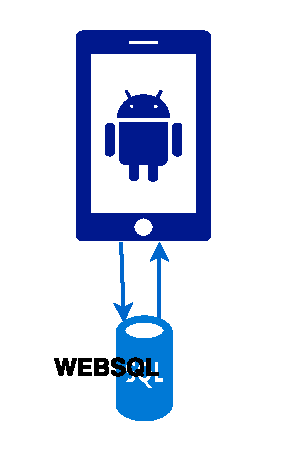
\includegraphics[width=0.3\textwidth]{DisenoOffline}
\captionsetup{justification=centering, margin=2cm}
\caption{Dise'no aplicaci'on movil y base de datos, Fuente: Elaboraci'on Propia}
\label{fig:DO}
\end{figure}

\subsection{El tercer etapa de la implementaci'on}
Para modificar la planilla de notas, sin conexi'on a internet, anteriormente ha debido crear su sesi'on y descargar la planilla de notas se utiliza localmente como se muestran a continuaci'on:
\begin{itemize}
\item Se utiliza el pouchdb y websql para crear, actualizar y modificar la base de datos se realizan en el archivo www/js/fileService.js.
\begin{verbatim}
.service('SagaaService', function($q) {
......
_db = new PouchDB('sagaa', { adapter: 'websql' }, 
 { skip_setup: true });//crear base de datos
 ......
  return $q.when( _db.post( sagaa));//añadir
  ......
  return $q.when(_db.put(sagaa));//actualizar
   .......
\end{verbatim}
\item Se guardan las solicitudes del servicio que tienen alg'un problema con la conecci'on o respuestas err'oneas, esto se ha realizado en el archivo app.js.
\begin{verbatim}
.....
//crea un interceptor
$httpProvider.interceptors.push('myInterceptor');
.....
//crear un interceptor
//crear metodo, para conocer la respuesta o la peticion
var interceptor = function ($q, logHttp) {
return {
  responseError: function(rejection) {
  logHttp.push(rejection.config);
  ......
  return $q.reject(rejection);
  ......}
}
\end{verbatim}
\item Guardar y verificar las peticiones al servicio se ha realizado en el fileService.js  
\begin{verbatim}
.service('myInterceptor', function($q, $timeout, logHttp){
return { 
	'request': function(config){ 
	......//guardamos la peticion sin error
	logHttp.push(config);
	.....
	'requestError': function(rejection){
	//guarda la peticion con error, 
	window.localStorage.setItem('id_request', data);
	......// lo mismo realiza en la respuesta con error
	.......
.service('logHttp', function($q) {
	push: function(config) {
	requestsConfig = config;
.............
\end{verbatim}
\end{itemize}

%desde aqui comienza
%En este c'apitulo se utilizan los datos obtenidos, del c'apitulo \ref{capituloseis} y se explican las herramientas que se utilizan para la implementaci'on de la aplicacion m'ovil y el desarrollo del mismo.


